%==========================================================
%-------------------- begin preamble ----------------------
%==========================================================
%\documentclass[12pt]{article}
\documentclass[12pt, a4paper, abstracton]{scrartcl}
\setkomafont{disposition}{\normalfont\bfseries}
\usepackage{setup/style}
%---------------- custom style -----------------------
%----- equation numbering -------
\numberwithin{equation}{section}     % number within section
%\numberwithin{equation}{subsection} % number within subsection


%----- fig & table numbering -----
\counterwithin{figure}{section}
\counterwithin{table}{section}

%--------- format abstract ---------
\makeatletter
\renewenvironment{abstract}{
    \if@twocolumn
      \section*{\abstractname}
    \else
      \begin{center}
        {\bfseries \large\abstractname\vspace{\z@}}
      \end{center}
      \quotation
    \fi}
    {\if@twocolumn\else\endquotation\fi}
\makeatother

%----------------- tikz ---------------------------
% Define block styles
\tikzstyle{startstop} = [rectangle, rounded corners,
    minimum width=3cm, minimum height=1cm,text centered, draw=black, fill=red!30]
\tikzstyle{io} = [trapezium, trapezium left angle=70, 
    trapezium right angle=110, minimum width=3cm, minimum height=1cm, text centered, text width=3cm, draw=black, fill=blue!30]
\tikzstyle{process} = [rectangle, minimum width=3cm,
    minimum height=1cm, text centered, text width=3cm, 
    draw=black, fill=orange!30] 
\tikzstyle{decision} = [diamond, minimum width=3cm, 
    minimum height=1cm, text centered,text width=2cm, 
    draw=black, fill=green!30]
\tikzstyle{arrow} = [thick,->,>=stealth]
\tikzstyle{block} = [rectangle, draw, fill=blue!20, 
    text width=5em, text centered, rounded corners, minimum height=4em]
\tikzstyle{line} = [draw, -latex']
\tikzstyle{cloud} = [draw, ellipse,fill=red!20, node distance=3cm,
    minimum height=2em]


%---------- insert custom LaTeX commands ----------
\newcommand*{\QED}{\hfill\ensuremath{\square}}
\newcommand{\e}{\mathrm{e}}
\newcommand{\E}{\mathrm{E}}
\newcommand{\R}{\mathbb{R}}
\newcommand{\X}{\mathbf{X}}
\newcommand{\y}{\mathbf{y}}
\newcommand{\rss}{\mathrm{RSS}}
\newcommand{\MSE}{\mathrm{MSE}}
\newcommand{\Err}{\mathrm{Err}}
\newcommand{\err}{\mathrm{err}}
\newcommand{\bias}{\mathrm{Bias}}
\newcommand{\Var}{\mathrm{Var}}
\DeclareMathOperator*{\argmax}{arg\,max}
\DeclareMathOperator*{\argmin}{arg\,min}
\DeclareMathOperator*{\cv}{CV}
\DeclareMathOperator*{\df}{df}
\newcommand{\T}{\mathcal{T}}

\NewDocumentCommand{\cw}{v}{%
\textbf{\texttt{\textcolor{Blue}{#1}}}%
}


\addbibresource{bibliography.bib}   % Bibliography

% Set graphics path
\graphicspath{{latex/figures/}}

%-------- header & foot -------- 
% FILL IN APPROPRIATE DESCRIPTIONS
% title page
\pagestyle{fancy}
\fancypagestyle{firststyle}
{
   \fancyhf{}
   \fancyfoot[C]{
   % Link to GitHub
   \faGithub \ 
   \href{https://github.com/nicolossus/FYS9429-Project1}{github.com/nicolossus/FYS9429-Project1}}
   \renewcommand{\headrulewidth}{0pt}
   \renewcommand{\footrulewidth}{0.4pt}
}
% rest of document
\fancyhead[L]{\small FYS5429/9429}       % Set <course>
\fancyhead[C]{\small Project 1}             % Set <title>    
\fancyhead[R]{\small March 22, 2024}   % Set <date>
\fancyfoot[C]{-- \thepage\ --}
\renewcommand{\headrulewidth}{0.4pt}
\renewcommand{\footrulewidth}{0.4pt}

% No header:
%\fancyhead{} 
%\renewcommand{\headrulewidth}{0pt}
\usepackage{appendix}
\AtBeginEnvironment{appendices}{\crefalias{section}{appendix}}

%==========================================================
%-------------------- end preamble ----------------------
%==========================================================

%==========================================================
%-------------------- main content ----------------------
%==========================================================
\begin{document}
%------------------ title -------------------------
%================================================================
%------------------------ Title Page ----------------------------
%================================================================
\newcommand{\horrule}[1]{\rule{\linewidth}{#1}} %Horizontal rule
\newcommand{\RNum}[1]{\uppercase\expandafter{\romannumeral #1\relax}}
\titlehead{
\includegraphics[scale=0.35]{latex/latex-report/Images/Logo/FI/MN_FYSISK_Seal_A_ENG.pdf}}
\title{
\large \textsc{FYS5429/9429: Advanced machine learning and data analysis for the physical sciences} % Set <COURSE>
\\ [25pt]
\horrule{0.5pt} \\[0.4cm]
\huge Project 1}               % Set <TITLE>
\subtitle{Neural sampling machine    % Set <SUBTITLE>
\horrule{2pt} \\[0.5cm]}
\author{Janita Ovidie Sandtrøen Willumsen \and Jan Fredrik Kismul \and Nicolai Haug}            % Set <AUTHOR>, separate multiple                                 % authors with \and
\date{March 22, 2024}     % Set <DATE>

\maketitle



\pagenumbering{gobble}
\thispagestyle{firststyle}

%---------------- abstract -------------------------
%================================================================
%------------------------- Abstract -----------------------------
%================================================================
\begin{abstract}

\end{abstract}
   % Abstract on title page
\newpage

%------------ content overview ---------------------
\frontmatter      % Folios in Roman numerals
\tableofcontents    
%\abstractintoc   % Add abstract to table of contents
%\listoffigures      
%\listoftables       
%\listofalgorithms
%\listoftodos       % list TODOs

%----------------- body ----------------------------
\mainmatter         % Folios in Arabic numerals
%================================================================
\section{Introduction}\label{sec:Introduction}
%================================================================

When working with high-dimensional data, analysis and modeling often necessitate the compression of the data into a lower-dimensional representation. It is then crucial to extract the relevant information. The features of high-dimensional data can be expertly crafted using domain knowledge or found by tapping into the ability of modern machine learning methods to learn useful representations of the data directly.

In this project, the objective is to investigate whether variational autoencoders (VAEs) \citep{kingma2022autoencoding} can be used to learn features from simulated neural recordings with the Hodgkin-Huxley model \citep{HH1952}. We embark on this quest in the traditional way -- by building simple models and testing them on the (binarized) MNIST dataset. Specifically, we will build VAEs with simple dense and convolutional neural networks as encoder/decoder architecture. In addition to reducing the dimensionality, it is desirable for the VAE to be able to extract meaningful and independent latent factors that explain the majority of the variation in the data. This is called disentangling the latent space and is facilitated by, for example, $\beta$-VAEs \citep{higgins2017betavae}. We will also build $\beta$-VAEs to explore the disentanglement of the latent space. Informed by experiments on the binarized MNIST dataset, we apply the VAEs on the the simulated neural data.

The report is organized as follows. In \autoref{sec:Theory} we first provide the theoretical background of variational autoencoders and the dense and convolutional neural networks we use as encoder/decoder architectures. We also provide some brief background necessary to understand the neural data on which we ultimately will train the VAE model. In \autoref{sec:Method} we present the datasets and the different VAE architectures used, as well as a short description of the methods applied in the training of the VAEs. In \autoref{sec:Results} we present and discuss the results. Finally, in \autoref{sec:Conclusion} we provide conclusions to the approach and outline possible avenues for future research.

\input{sections/4_theory}
%================================================================
\section{Methodology}\label{sec:Method}
%================================================================

%----------------------------------------------------------------
\subsection{Sampling Algorithms}\label{sec:sampling_algos}
%----------------------------------------------------------------

\begin{itemize}
    \item MNIST, HH
    \item FFNN-VAE
    \item Conv-VAE
    \item Difference in loss when using MNIST (cross-entropy) and HH (MSE)
    \item $\beta$-VAE
    \item LSTM-based VAE
    \item Latent perturbation
\end{itemize}

\newpage
%================================================================
\section{Results and Discussion}\label{sec:Results}
%================================================================

\subsection{Binarized MNIST experiments}

\subsubsection{The effect of the latent dimension}  

\autoref{fig:loss_latent_dim_vanilla_vae_bmnist} show the ELBO ... during training for different choices of latent dimensions. In terms of the loss, the Conv-VAE generally performs slightly better than the MLP- and DNN-VAE.
why? cnn in principle better at extracting features 

\begin{figure}[!htb]
\begin{center}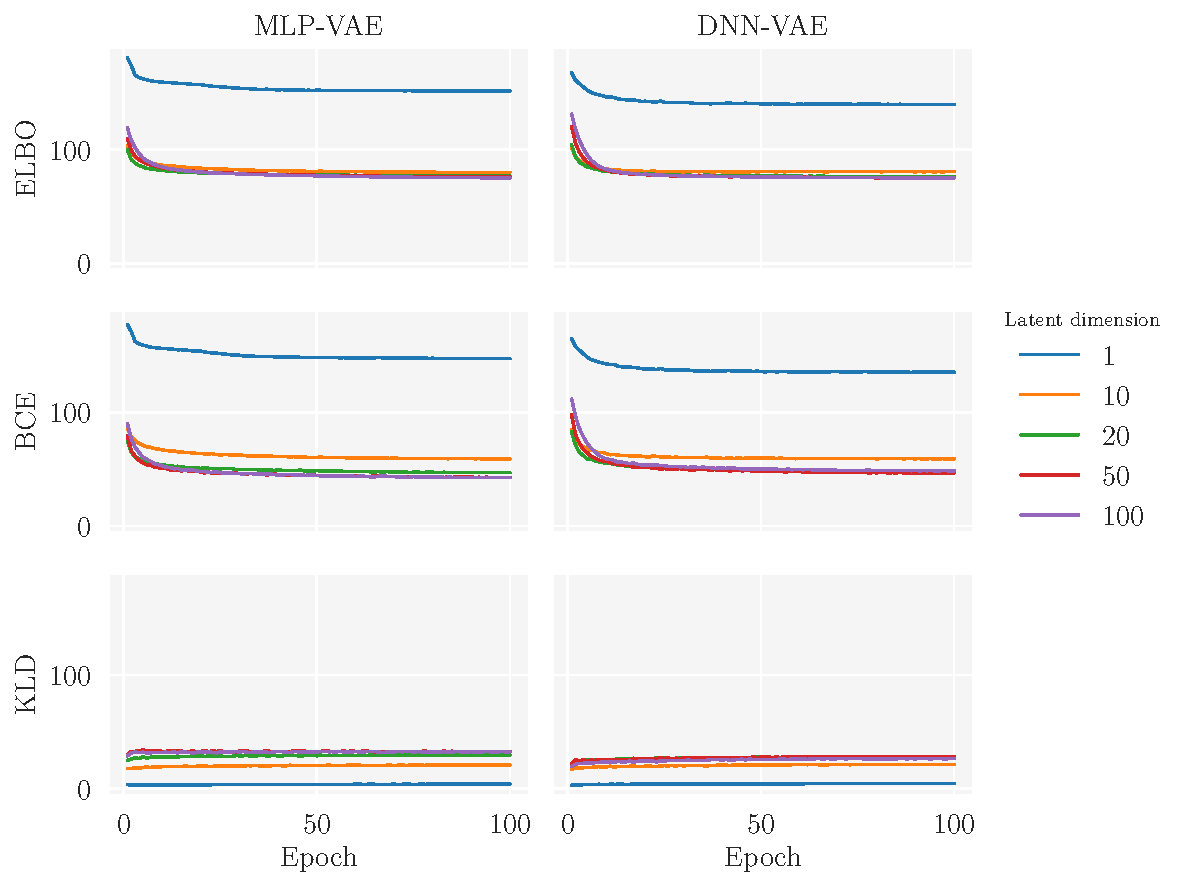
\includegraphics[scale=0.75]{latex/figures/loss_latent_dim_vanilla_mlp_dnn_vae_bmnist.pdf}
\end{center}
\caption{figure text}
\label{fig:loss_latent_dim_vanilla_vae_bmnist}
\end{figure}

\autoref{fig:recon_latent_dim_vanilla_vae_bmnist} shows the VAEs reconstructed images from the test set.

\begin{figure}[!htb]
\centering
\subfloat[]{{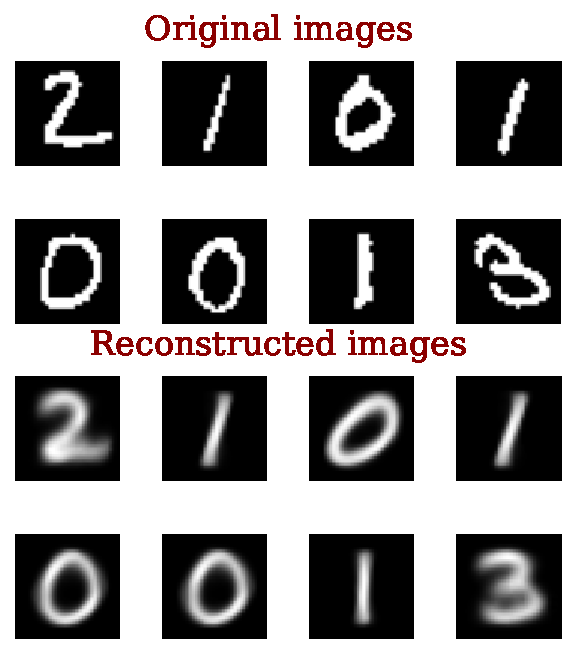
\includegraphics[scale=0.5]{latex/figures/recon_latent_dim_1_vanilla_mlp_vae_bmnist.pdf}}}
\qquad
\subfloat[]{{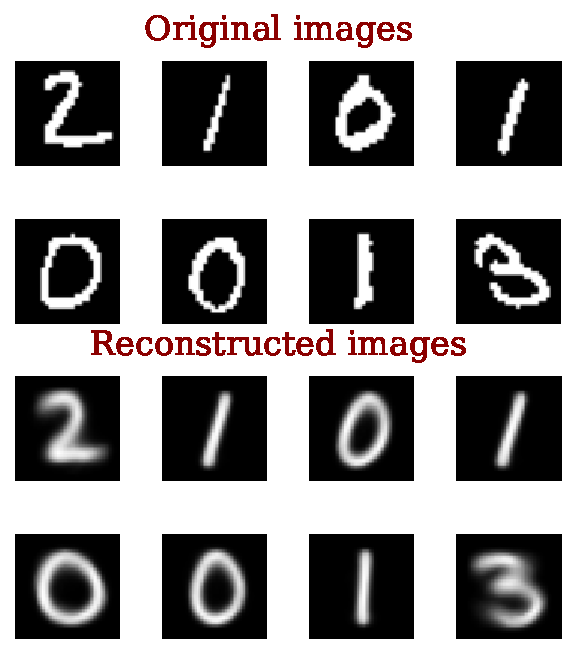
\includegraphics[scale=0.5]{latex/figures/recon_latent_dim_1_vanilla_dnn_vae_bmnist.pdf}}}
\qquad
\subfloat[]{{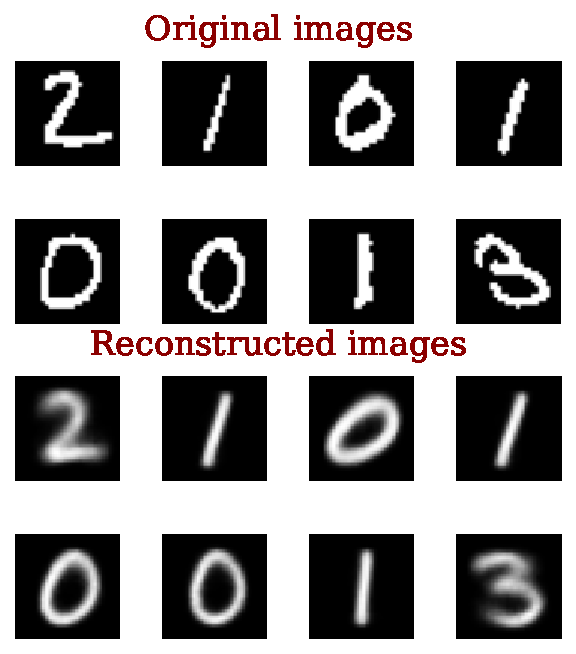
\includegraphics[scale=0.5]{latex/figures/recon_latent_dim_1_vanilla_conv_vae_bmnist.pdf}}}
\qquad
\subfloat[]{{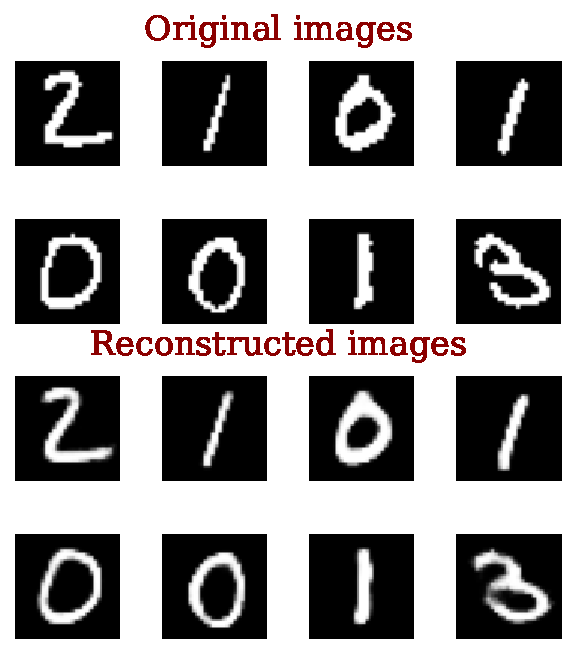
\includegraphics[scale=0.5]{latex/figures/recon_latent_dim_20_vanilla_mlp_vae_bmnist.pdf}}}
\qquad
\subfloat[]{{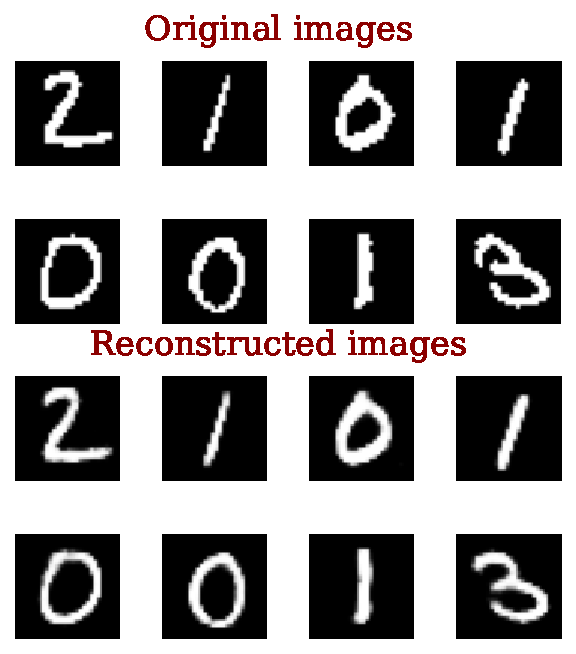
\includegraphics[scale=0.5]{latex/figures/recon_latent_dim_20_vanilla_dnn_vae_bmnist.pdf}}}
\qquad
\subfloat[]{{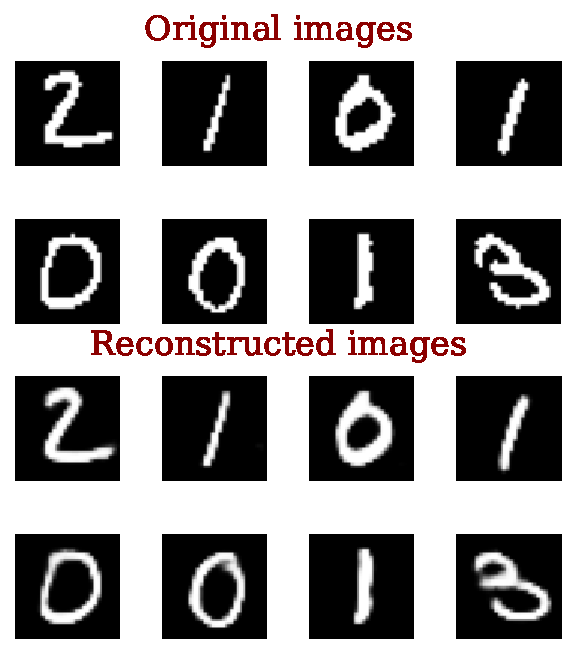
\includegraphics[scale=0.5]{latex/figures/recon_latent_dim_20_vanilla_conv_vae_bmnist.pdf}}}
\qquad
\subfloat[]{{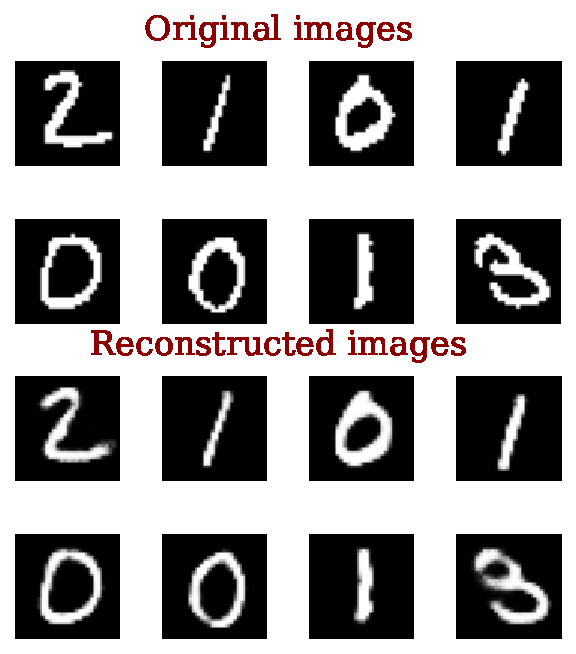
\includegraphics[scale=0.5]{latex/figures/recon_latent_dim_100_vanilla_mlp_vae_bmnist.pdf}}}
\qquad
\subfloat[]{{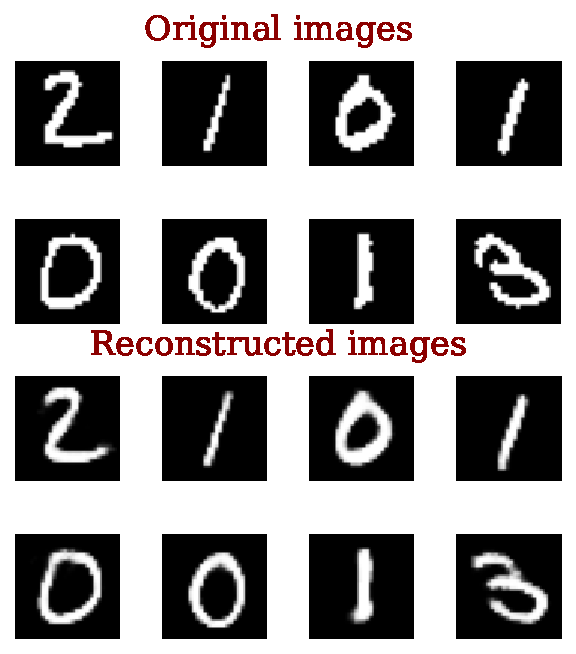
\includegraphics[scale=0.5]{latex/figures/recon_latent_dim_100_vanilla_dnn_vae_bmnist.pdf}}}
\qquad
\subfloat[]{{
\includegraphics[scale=0.5]{latex/figures/recon_latent_dim_100_vanilla_conv_vae_bmnist.pdf}}}
\caption{Comparison of original and reconstructed images. Grids to the left are the MLP-VAE, in the middle DNN-VAE and to the right Conv-VAE. The top row shows 1 latent dimension, the middle 20 latent dimensions and the bottom 100}
\label{fig:recon_latent_dim_vanilla_vae_bmnist}
\end{figure}


\autoref{fig:samples_latent_dim_vanilla_vae_bmnist} shows generated samples

\begin{figure}[!htb]
\centering
\subfloat[]{{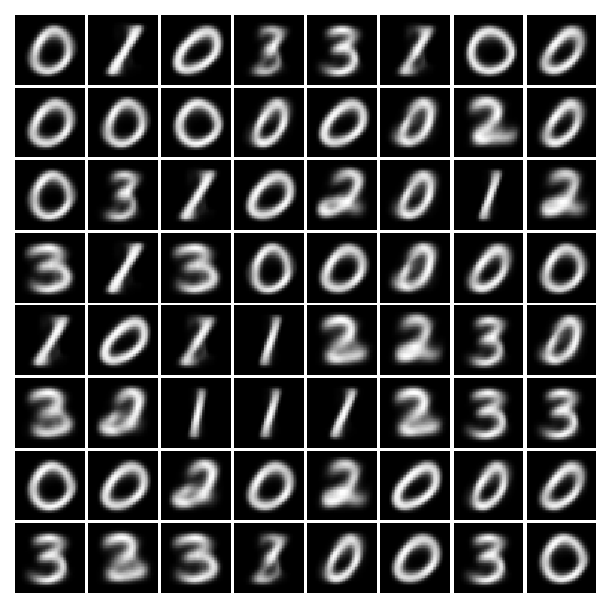
\includegraphics[scale=0.45]{latex/figures/samples_latent_dim_1_vanilla_mlp_vae_bmnist.pdf}}}
\qquad
\subfloat[]{{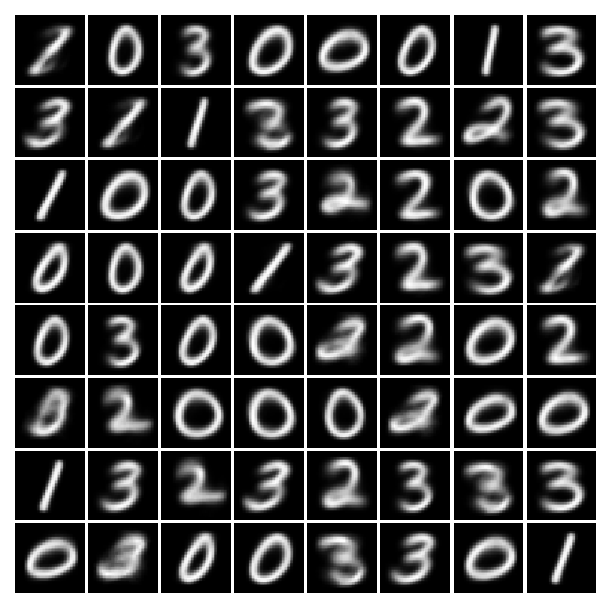
\includegraphics[scale=0.45]{latex/figures/samples_latent_dim_1_vanilla_dnn_vae_bmnist.pdf}}}
\qquad
\subfloat[]{{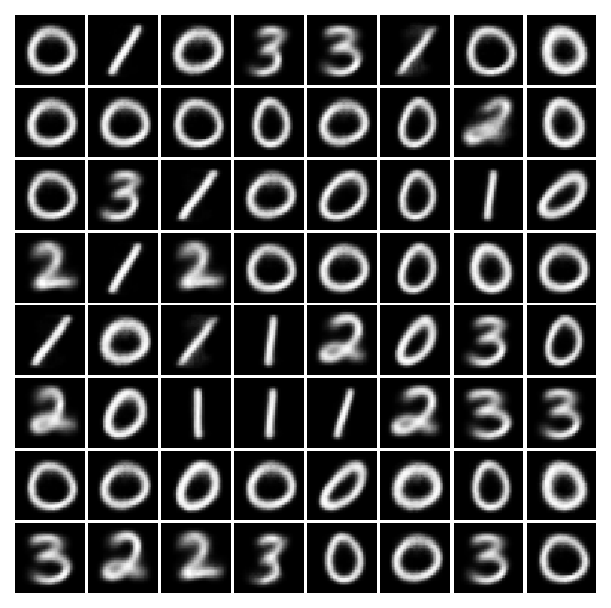
\includegraphics[scale=0.45]{latex/figures/samples_latent_dim_1_vanilla_conv_vae_bmnist.pdf}}}
\qquad
\subfloat[]{{
\includegraphics[scale=0.45]{latex/figures/samples_latent_dim_20_vanilla_mlp_vae_bmnist.pdf}}}
\qquad
\subfloat[]{{
\includegraphics[scale=0.45]{latex/figures/samples_latent_dim_20_vanilla_dnn_vae_bmnist.pdf}}}
\qquad
\subfloat[]{{
\includegraphics[scale=0.45]{latex/figures/samples_latent_dim_20_vanilla_conv_vae_bmnist.pdf}}}
\qquad
\subfloat[]{{
\includegraphics[scale=0.45]{latex/figures/samples_latent_dim_100_vanilla_mlp_vae_bmnist.pdf}}}
\qquad
\subfloat[]{{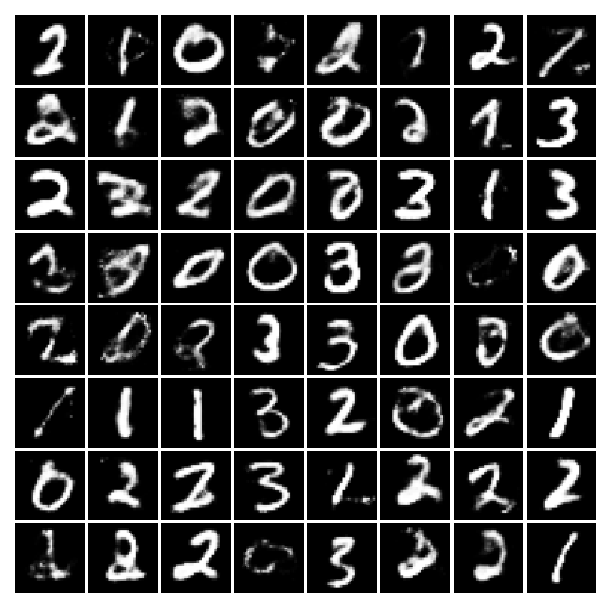
\includegraphics[scale=0.45]{latex/figures/samples_latent_dim_100_vanilla_dnn_vae_bmnist.pdf}}}
\qquad
\subfloat[]{{
\includegraphics[scale=0.45]{latex/figures/samples_latent_dim_100_vanilla_conv_vae_bmnist.pdf}}}
\caption{Comparison of original and reconstructed images. Grids to the left are the MLP-VAE, in the middle DNN-VAE and to the right Conv-VAE. The top row shows 1 latent dimension, the middle 20 latent dimensions and the bottom 100}
\label{fig:samples_latent_dim_vanilla_vae_bmnist}
\end{figure}





\FloatBarrier
\subsubsection{Disentangling the latent space}

\autoref{fig:beta_vae_tradeoff}
\begin{figure}[!htb]
\begin{center}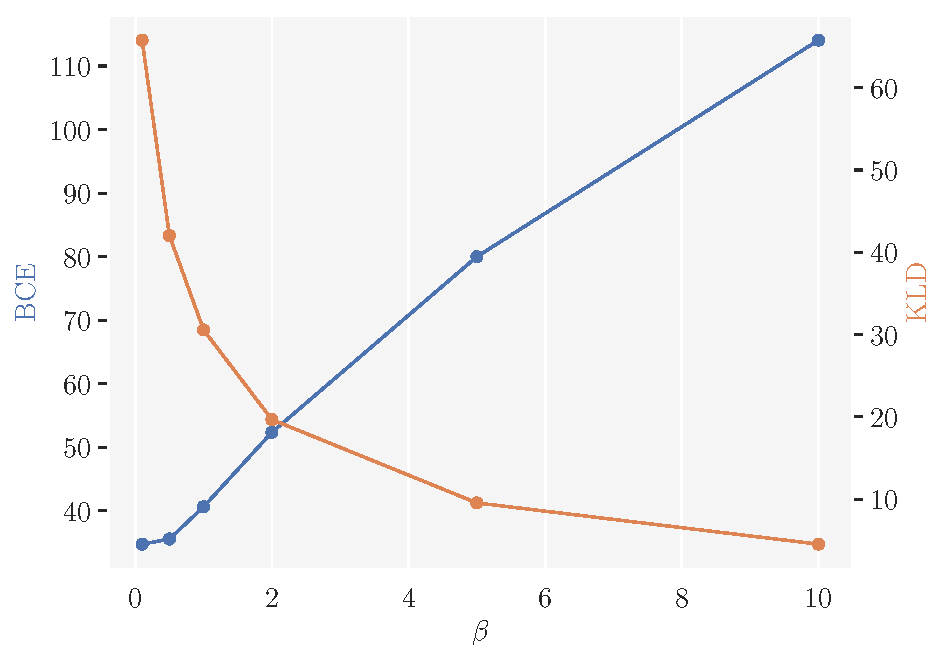
\includegraphics[scale=0.75]{latex/figures/bce_kld_vs_beta.pdf}
\end{center}
\caption{figure text}
\label{fig:beta_vae_tradeoff}
\end{figure}

\autoref{fig:tsne_beta_vae_bmnist} shows the t-SNE embedding of the latent distribution for different values of $\beta$. The color and label of each cluster corresponds to the MNIST digit label. .. on test set

\begin{figure}[!htb]
\centering
\subfloat[]{{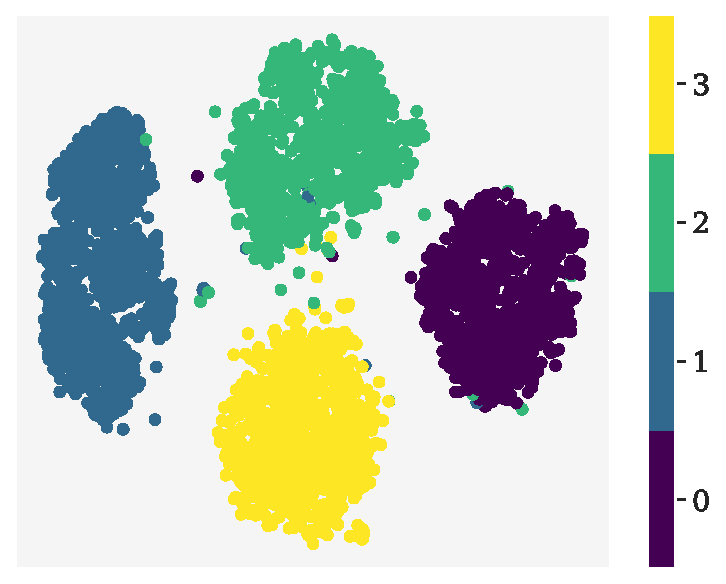
\includegraphics[scale=0.45]{latex/figures/tsne_beta_0.1_vae.pdf}}}
\qquad
\subfloat[]{{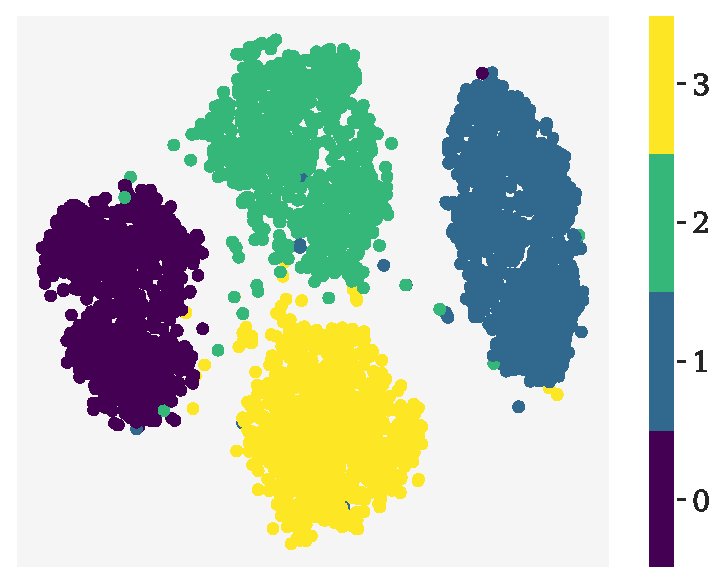
\includegraphics[scale=0.45]{latex/figures/tsne_beta_0.5_vae.pdf}}}
\qquad
\subfloat[]{{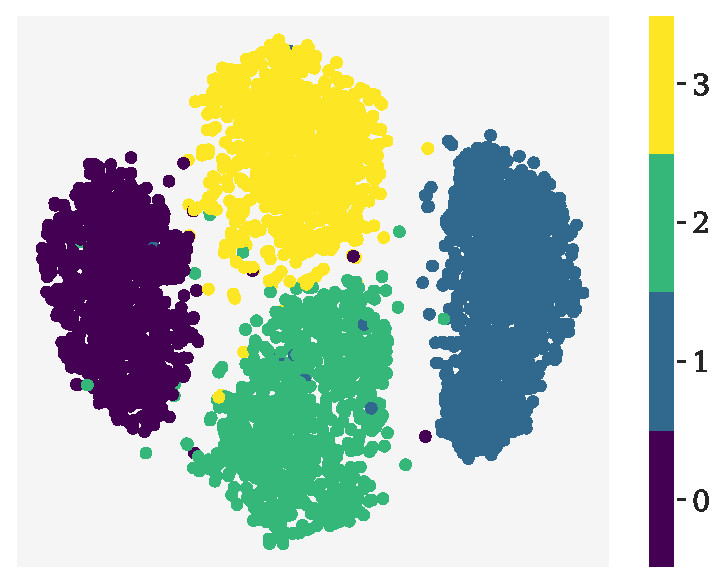
\includegraphics[scale=0.45]{latex/figures/tsne_beta_1_vae.pdf}}}
\qquad
\subfloat[]{{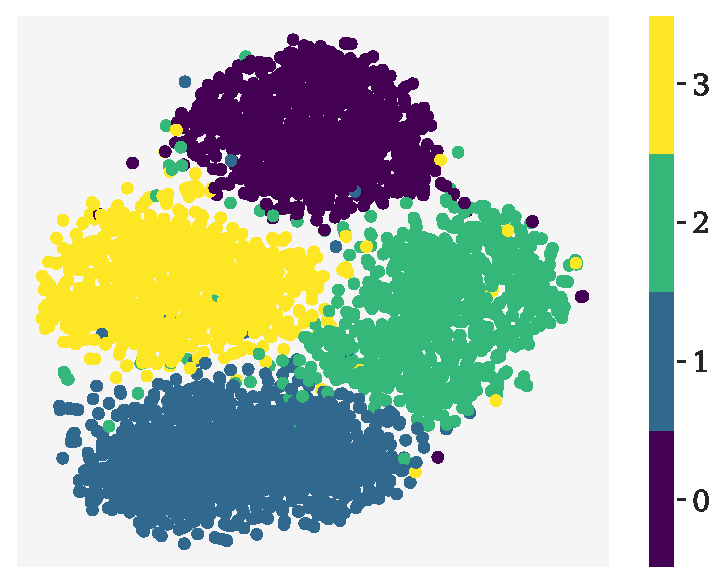
\includegraphics[scale=0.45]{latex/figures/tsne_beta_2_vae.pdf}}}
\qquad
\subfloat[]{{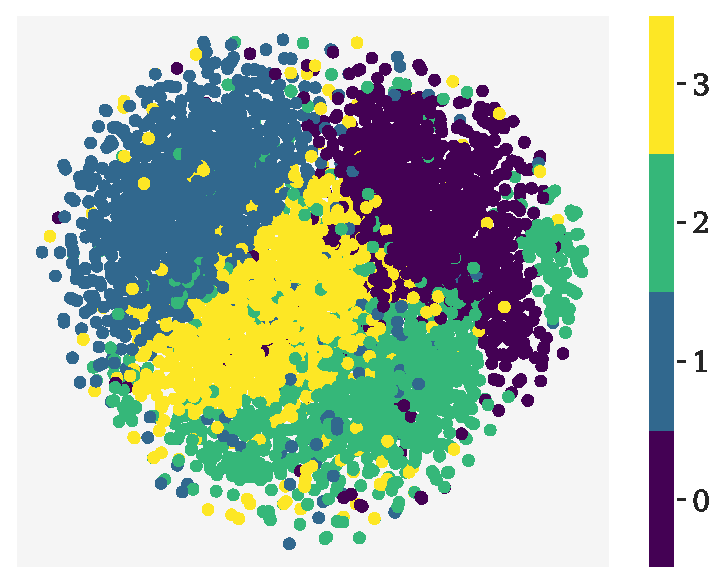
\includegraphics[scale=0.45]{latex/figures/tsne_beta_5_vae.pdf}}}
\qquad
\subfloat[]{{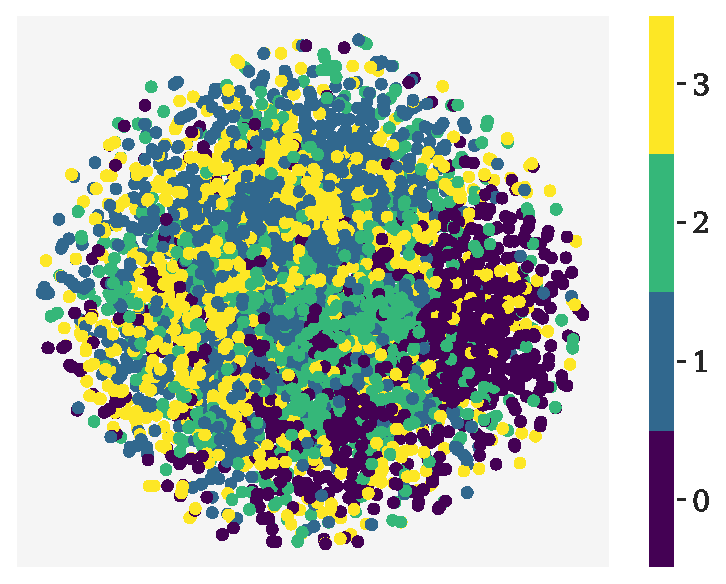
\includegraphics[scale=0.45]{latex/figures/tsne_beta_10_vae.pdf}}}
\caption{t-SNE }
\label{fig:tsne_beta_vae_bmnist}
\end{figure}

\FloatBarrier
%----------------------------------------------------------------
\subsection{Neural activity data experiments}
%----------------------------------------------------------------

\autoref{fig:hh_conv_vae_beta_1_z_20}

\begin{figure}[!htb]
\begin{center}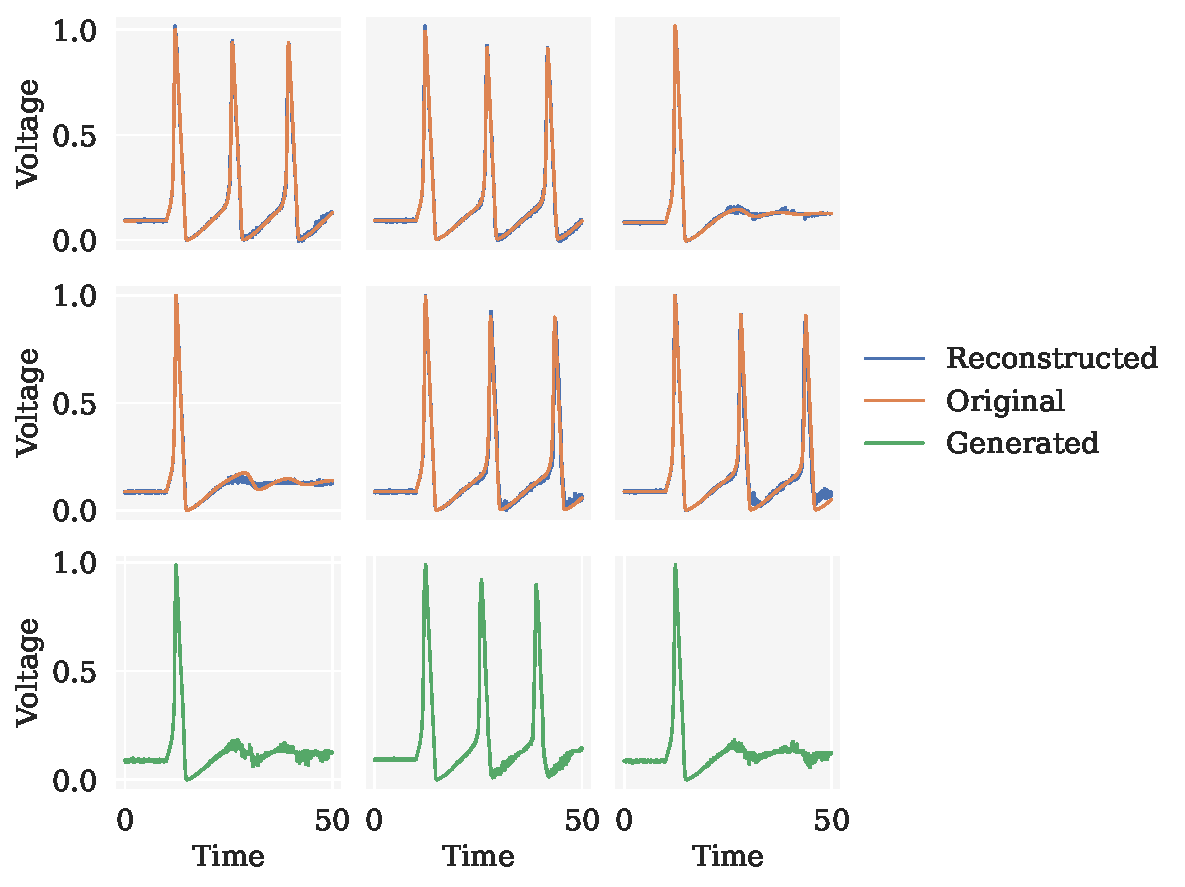
\includegraphics[scale=0.75]{latex/figures/hh_conv_vae_beta_1_z_20.pdf}
\end{center}
\caption{beta 1, z 20}
\label{fig:hh_conv_vae_beta_1_z_20}
\end{figure}

\autoref{fig:hh_conv_vae_beta_1_z_2_10}. See \autoref{fig:hh_conv_vae_beta_0_5} and \autoref{fig:hh_conv_vae_beta_2} for results with $\beta=0.5$ and $\beta=2$, respectively.


\begin{figure}[!htb]
\centering
\subfloat[]{{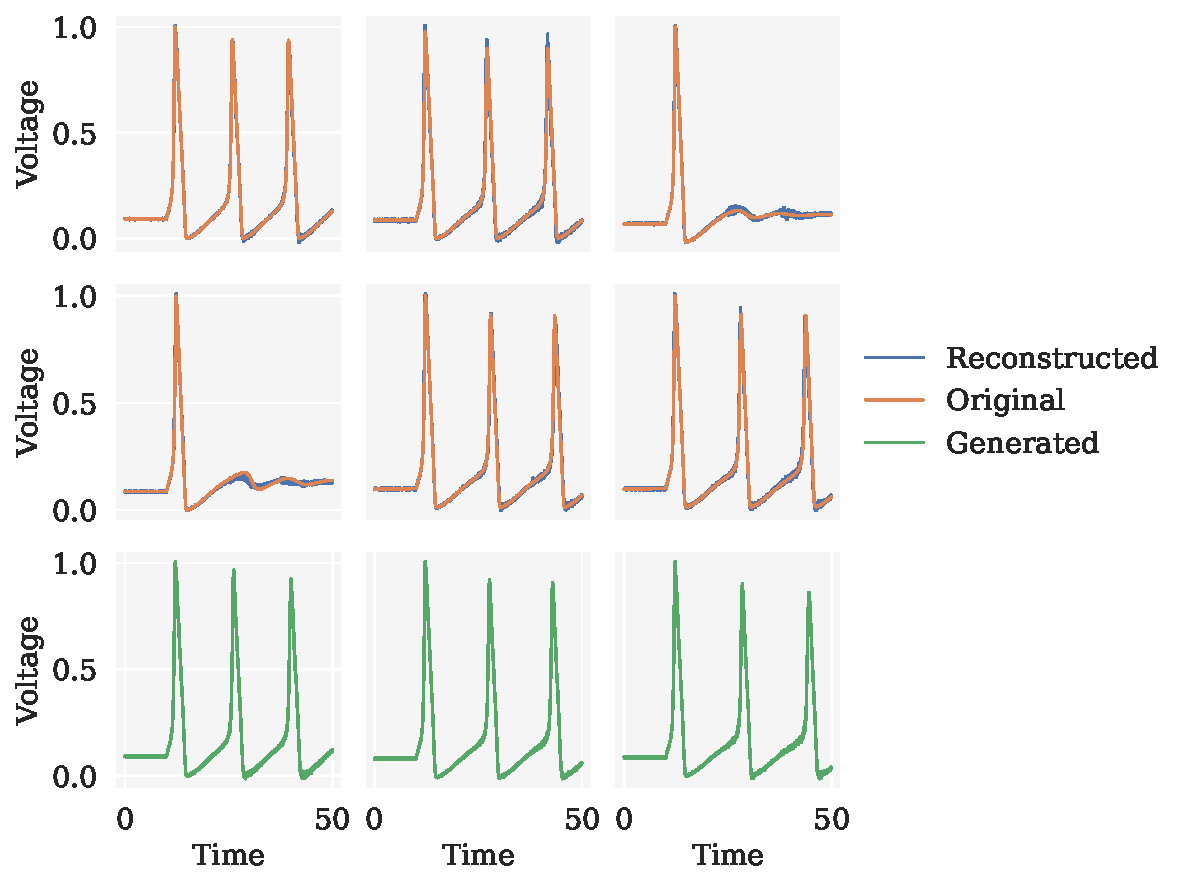
\includegraphics[scale=0.38]{latex/figures/hh_conv_vae_beta_1_z_2.pdf}}}
\qquad
\subfloat[]{{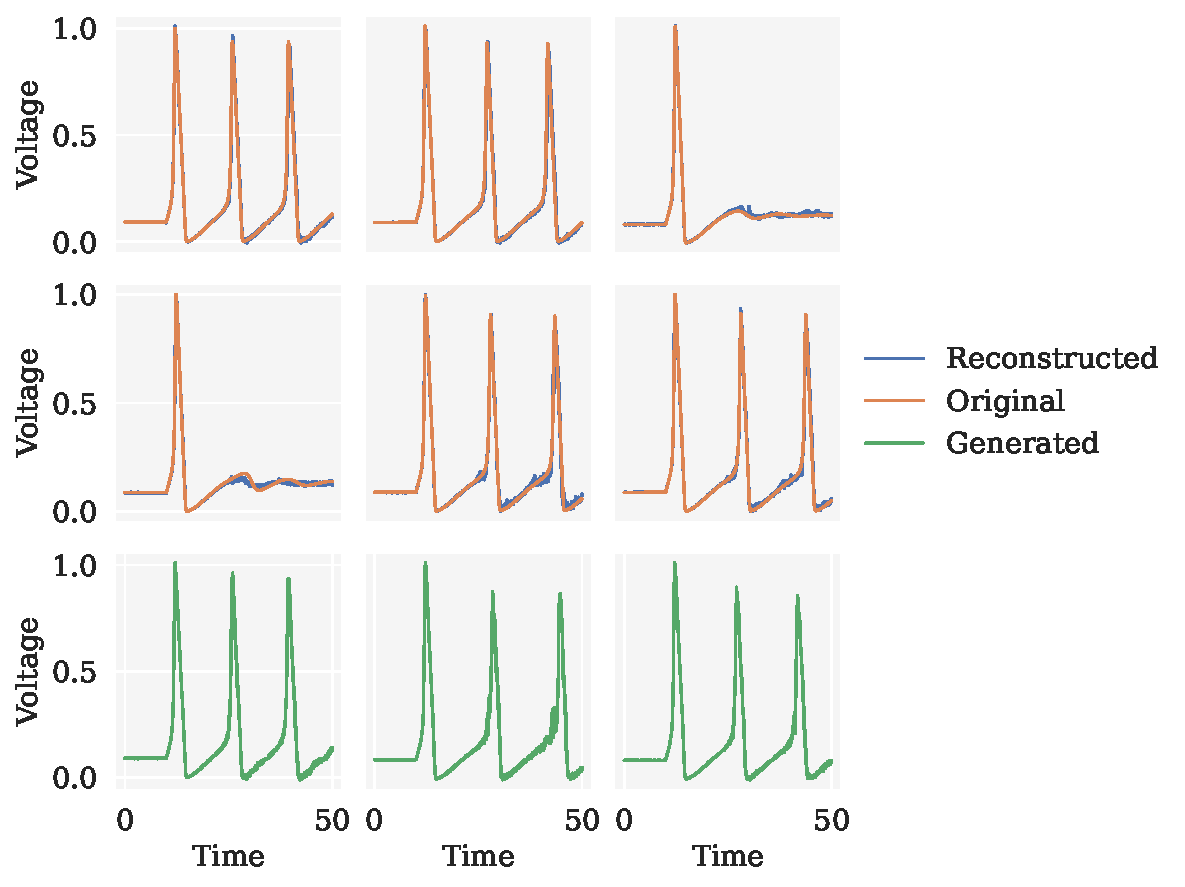
\includegraphics[scale=0.38]{latex/figures/hh_conv_vae_beta_1_z_10.pdf}}}
\caption{beta 1, z 2 10 }
\label{fig:hh_conv_vae_beta_1_z_2_10}
\end{figure}


%----------------------------------------------------------------
\subsection{Results 1}\label{sec:project results}
%----------------------------------------------------------------

%\FloatBarrier


\url{https://uvadlc-notebooks.readthedocs.io/en/latest/tutorial_notebooks/JAX/tutorial9/AE_CIFAR10.html}

% Comparing latent dimensionality

% When training an autoencoder, we need to choose a dimensionality for the latent representation. The higher the latent dimensionality, the better we expect the reconstruction to be. However, the idea of autoencoders is to compress data. Hence, we are also interested in keeping the dimensionality low. To find the best tradeoff, we can train multiple models with different latent dimensionalities. The original input has 32x32x3 = 3072 pixels. Keeping this in mind, a reasonable choice for the latent dimensionality might be between 64 and 384:

% Clearly, the smallest latent dimensionality can only save information about the rough shape and color of the object, but the reconstructed image is extremely blurry and it is hard to recognize the original object in the reconstruction. With 128 features, we can recognize some shapes again although the picture remains blurry. The models with the highest two dimensionalities reconstruct the images quite well. The difference between 256 and 384 is marginal at first sight but can be noticed when comparing, for instance, the backgrounds of the first image (the 384 features model more of the pattern than 256).

% The encoder and decoder networks we chose here are relatively simple. Usually, more complex networks are applied, especially when using a ResNet-based architecture. For example, see VQ-VAE and NVAE
%%================================================================
\section{Discussion}\label{sec:Discussion}
%================================================================

%----------------------------------------------------------------
\subsection{Project Discussion 1}\label{sec:project discussion}
%----------------------------------------------------------------

NOT IN USE
%================================================================
\section{Conclusion}\label{sec:Conclusion}
%================================================================


%================================================================
\section{Future Work}\label{sec:Future}
%================================================================


 
%-------- bibliography ----------- 
%\newpage 
\printbibliography[heading=bibintoc, title={References}]

%-------- appendix -----------
\appendix
%================================================================
\section{Appendix}\label{sec:Appendix A}
%================================================================

%----------------------------------------------------------------
\subsection{Additional Results}\label{app:additional_results}
%---------------------------------------------------------------- 


% hh_mse_kld_vs_beta_conv_vae.pdf

\autoref{fig:hh_conv_vae_beta_0_5} and \autoref{fig:hh_conv_vae_beta_2} are supplementary to \autoref{fig:hh_conv_vae_beta_1_z_20} and \autoref{fig:hh_conv_vae_beta_1_z_2_10}, and show the convolutional $\beta$-VAE's reconstructed and generated voltage traces for $\beta = 0.5$ and $\beta=2$, respectively, with $\dim (z) = \{2, 10, 20\}$.

\begin{figure}[!htb]
\centering
\subfloat[]{{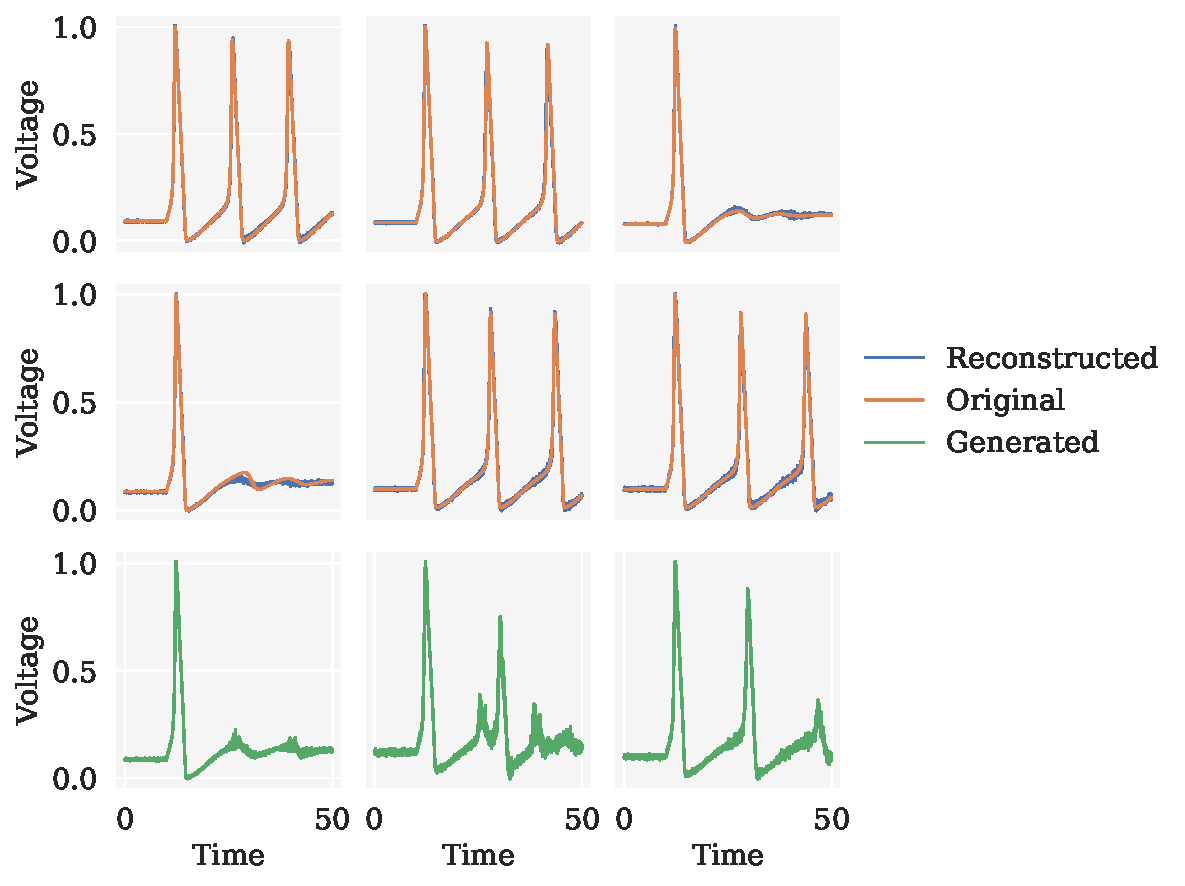
\includegraphics[scale=0.38]{latex/figures/hh_conv_vae_beta_0.5_z_2.pdf}}}
\qquad
\subfloat[]{{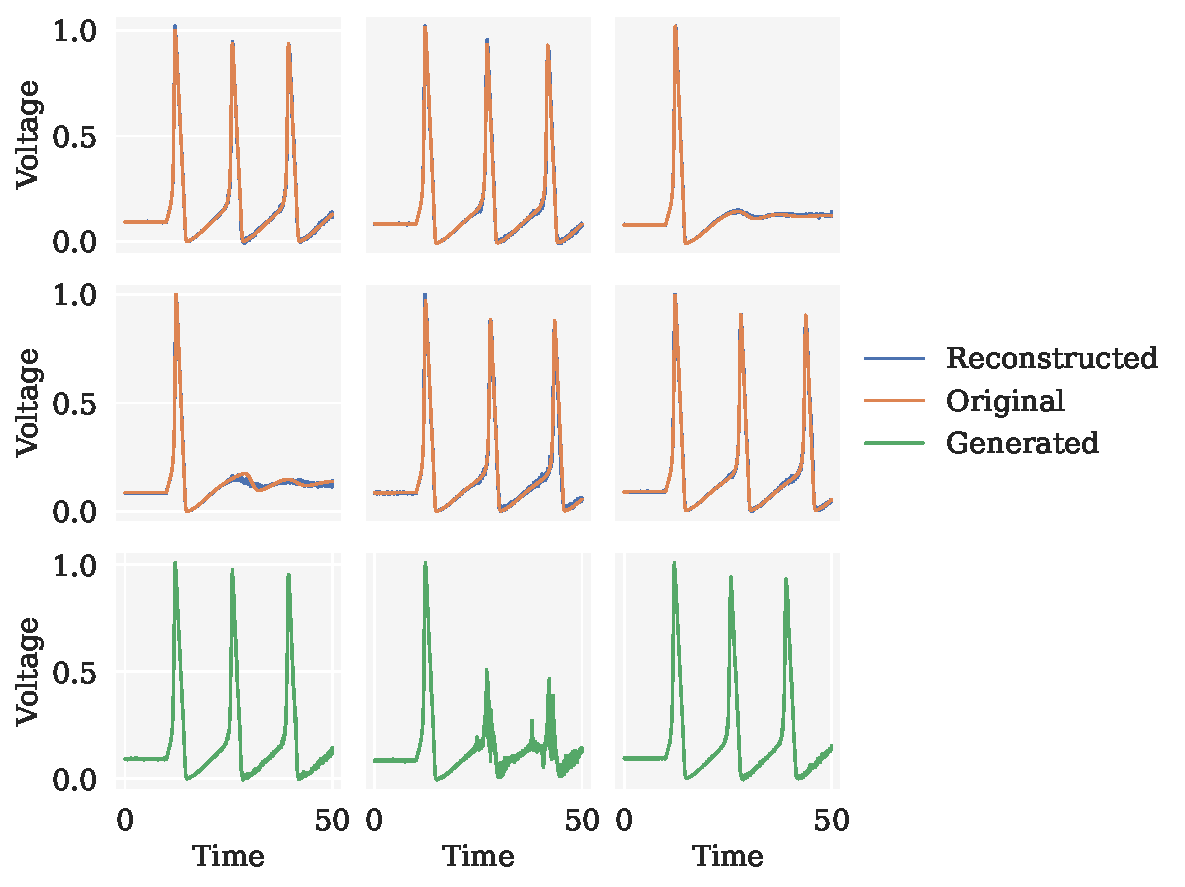
\includegraphics[scale=0.38]{latex/figures/hh_conv_vae_beta_0.5_z_10.pdf}}}
\qquad
\subfloat[]{{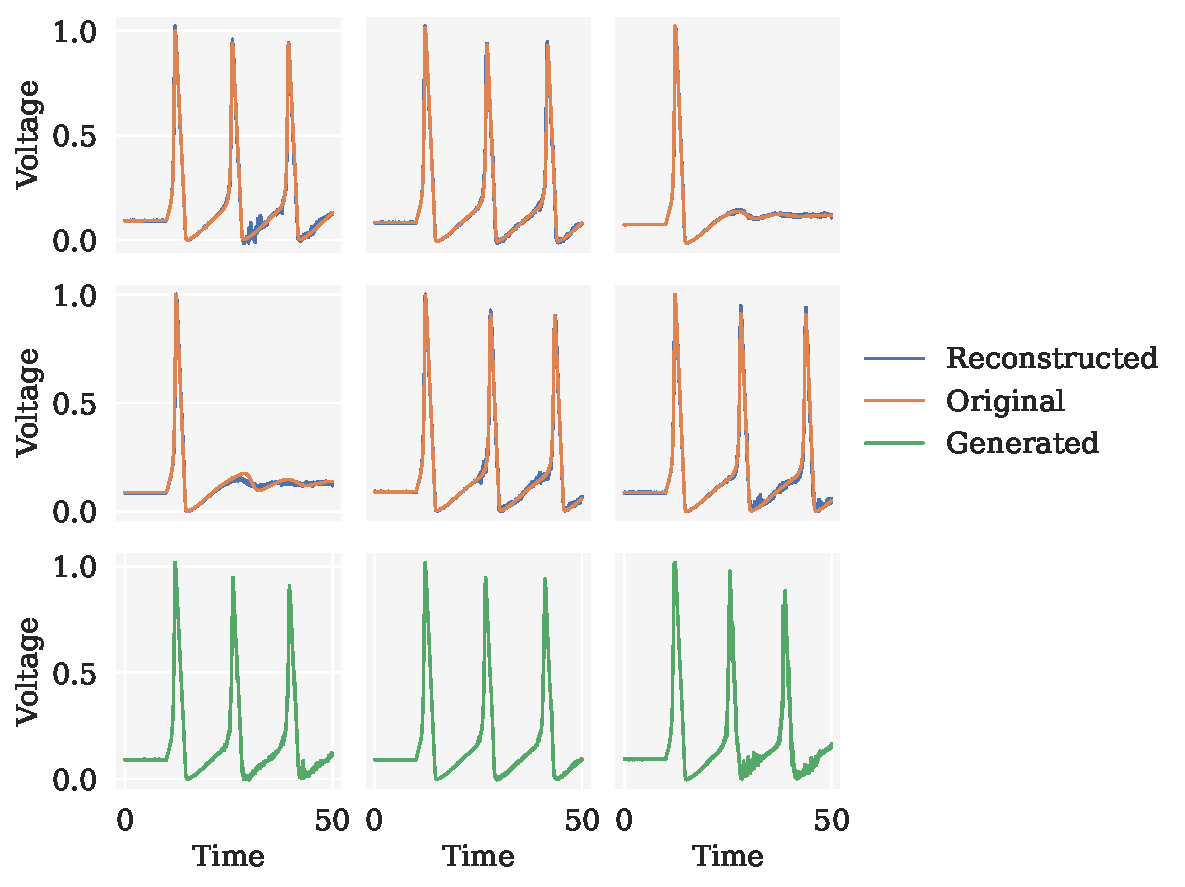
\includegraphics[scale=0.38]{latex/figures/hh_conv_vae_beta_0.5_z_20.pdf}}}
\caption{beta 0.5}
\label{fig:hh_conv_vae_beta_0_5}
\end{figure}

\begin{figure}[!htb]
\centering
\subfloat[]{{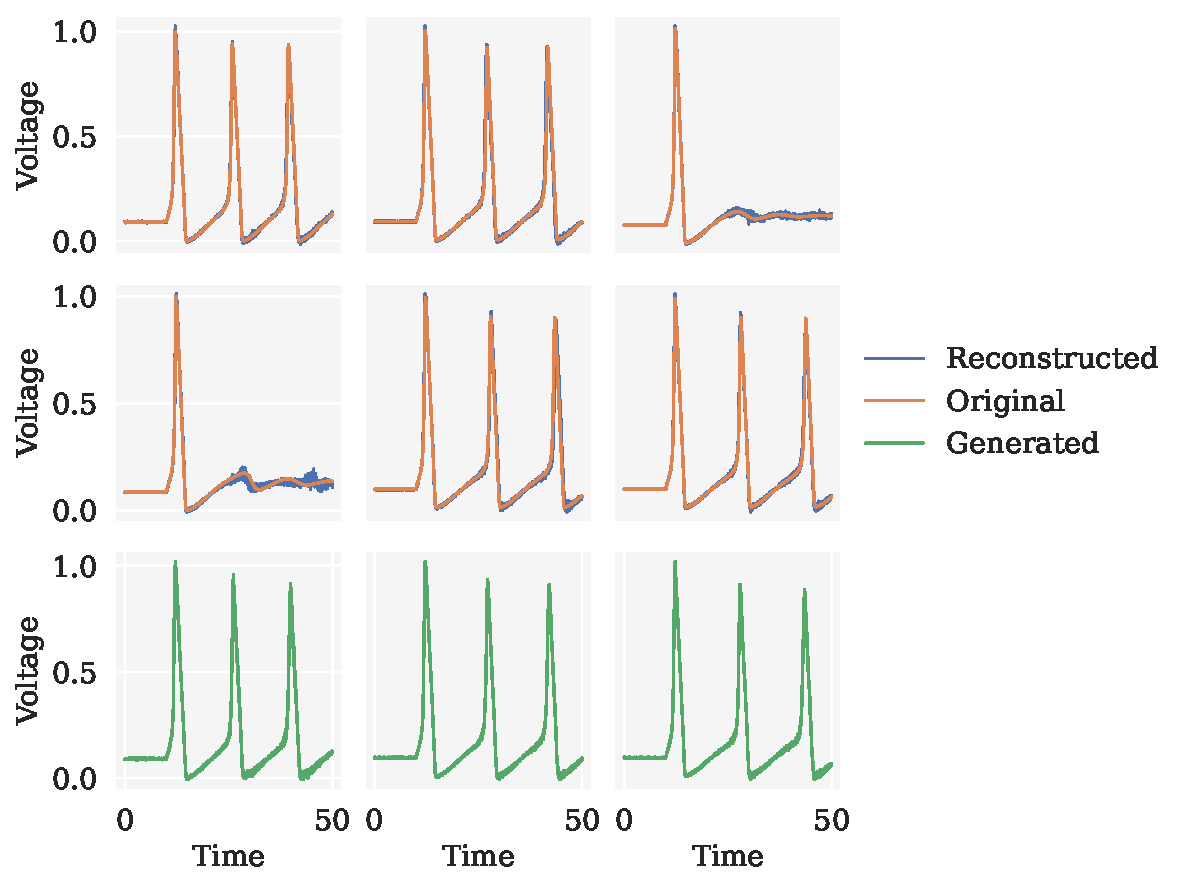
\includegraphics[scale=0.38]{latex/figures/hh_conv_vae_beta_2_z_2.pdf}}}
\qquad
\subfloat[]{{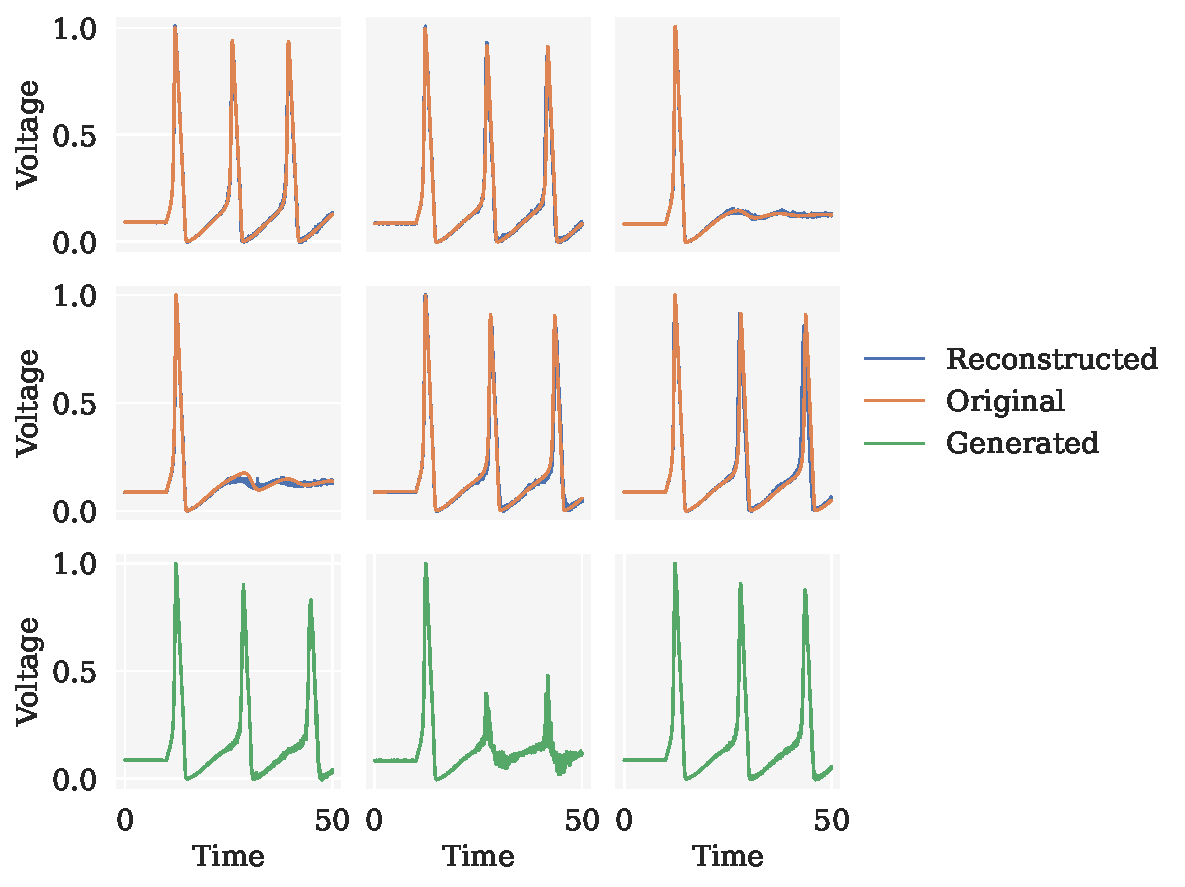
\includegraphics[scale=0.38]{latex/figures/hh_conv_vae_beta_2_z_10.pdf}}}
\qquad
\subfloat[]{{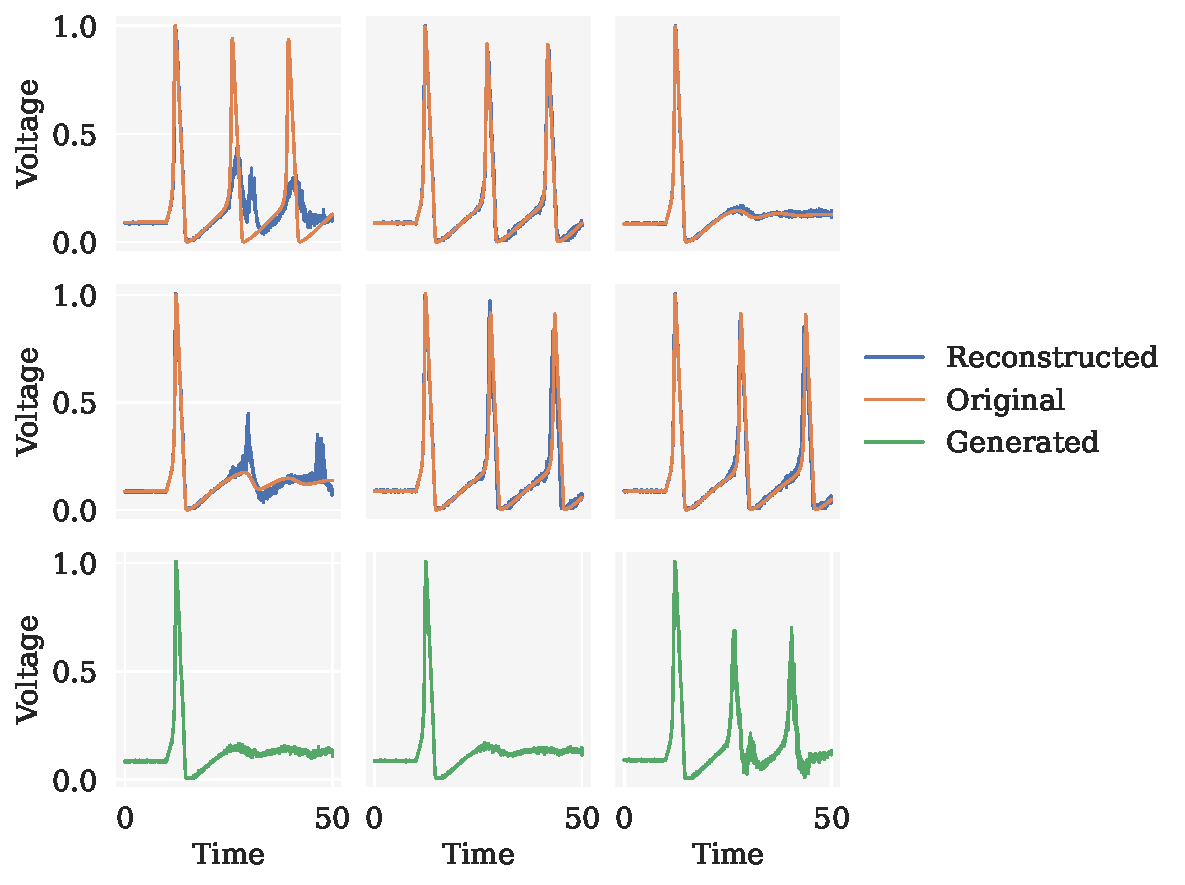
\includegraphics[scale=0.38]{latex/figures/hh_conv_vae_beta_2_z_20.pdf}}}
\caption{beta 2}
\label{fig:hh_conv_vae_beta_2}
\end{figure}
 

\end{document}
%==========================================================
% ------------------- end of main content ---------------
%==========================================================
